
The level of pixel noise present in galaxy images
greatly impacts the ability of lensing pipelines 
to accurately measure shear \citep[e.g.][]{peter_n, Okura_n, R_n}. 
The multiplicative bias due to pixel noise varies 
depending on both the source galaxy population
and the lensing pipeline. There have been a number
of schemes that attempt to correct for the
effect of noise bias for specific lensing pipelines
including \citet{K_n}, \citet{cfhtls}, and \citet{Bernstein2014}.  \\

To make the results easier to interpret and compare to previous
studies, the bias of the lensing pipelines was quantified in this
section by a linear function Eqn. \ref{Eqn:MC}.
The results of the multiplicative bias as a function of SNR are shown in Figure \ref{fig:Snr}. 
\begin{figure}
 \centering  % this centres figure in column
  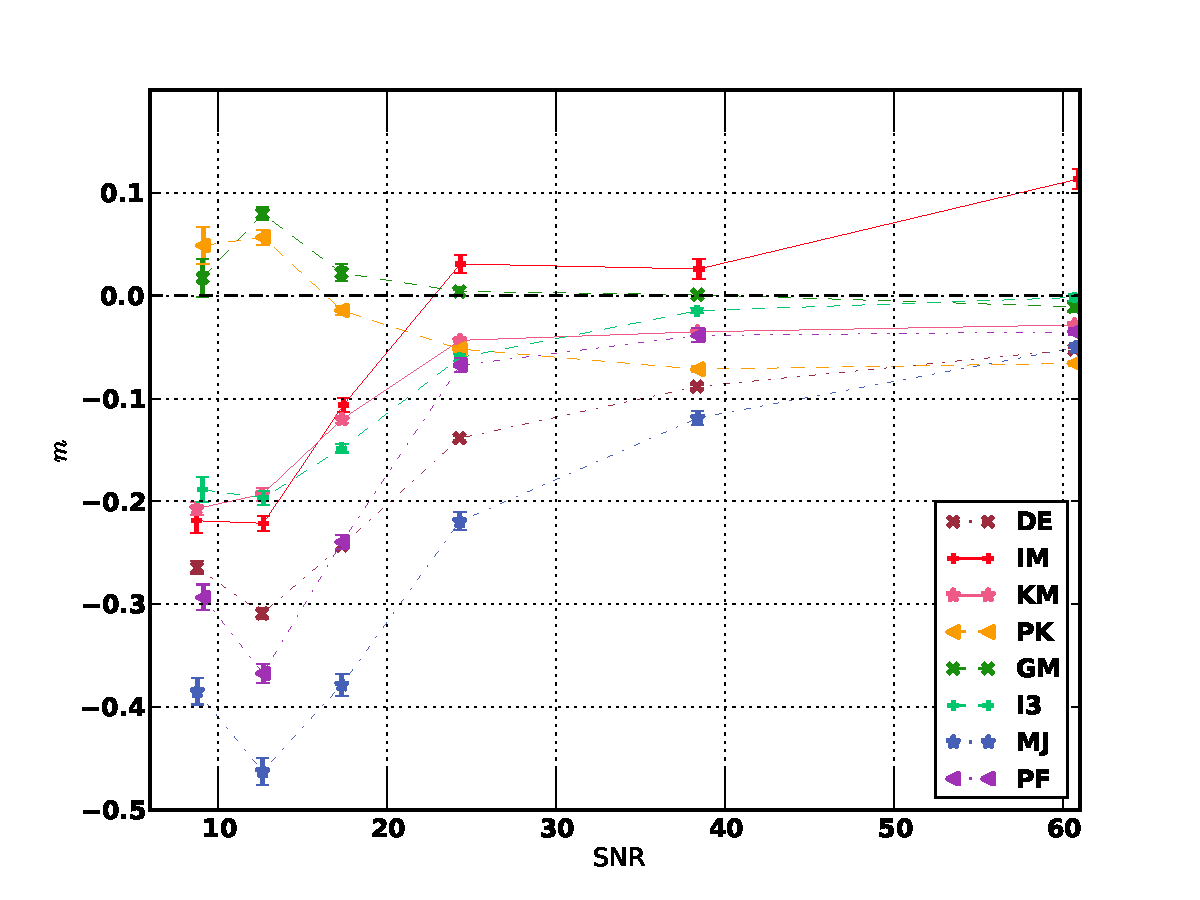
\includegraphics[width=0.5\textwidth]{fig/MvalSNR_v2.pdf} 
  \caption{Multiplicative bias ($m$) as a function
    of Signal-to-Noise Ratio (SNR). The multiplicative bias was determined
    using a linear fit of measured to true mean shear.}
\label{fig:Snr}
\end{figure}

\green{added this sentence of interpretation, which is still a bit on the stub side} The dependence of multiplicative biases on SNR are significant for most of the pipelines tested, but strongest in the regime of low SNR ($<20$). Careful calibration is therefore necessary if the shapes of these very faint galaxies are to be used in a weak lensing analysis.